\documentclass{beamer}
\usepackage{graphicx}\graphicspath{{../gfx/}}
%%%%%%%%%%%%%%%%%%%%%%%%%%%%%%%%%%%%%%%%%%%%%%%%%%%%%
% https://deic-web.uab.cat/~iblanes/beamer_gallery/ %
%%%%%%%%%%%%%%%%%%%%%%%%%%%%%%%%%%%%%%%%%%%%%%%%%%%%%
\usetheme{Warsaw}           % defaults to royal blue
% \usecolortheme[]{crane}   % example orange
% \usecolortheme[]{beaver}  % example
% Or define your own colortheme
\definecolor{myGreen}{rgb}{.125,.5,.25}
% \usecolortheme[named=myGreen]{structure}

\title[
  CDD Slide
  \insertframenumber/\inserttotalframenumber
  ]{Creditors Direct Debit}

\subtitle{Domiciliëring Schuldeiser}
\author{Jos Vermoesen}
\institute{Vsoft Administratieve Software}
\date{}

\begin{document}

\begin{frame}
  \begin{titlepage}
  \end{titlepage}
\end{frame}

% HINT: for less typing copy/paste frame template
% \begin{frame}[t]{Another Title name of my slide}\vspace{10pt}
%  Whatever
% \end{frame}

\begin{frame}[t]{De Toepassing}
  \begin{block}{APP Online}
    \vspace{0.5em}
    \begin{center}
      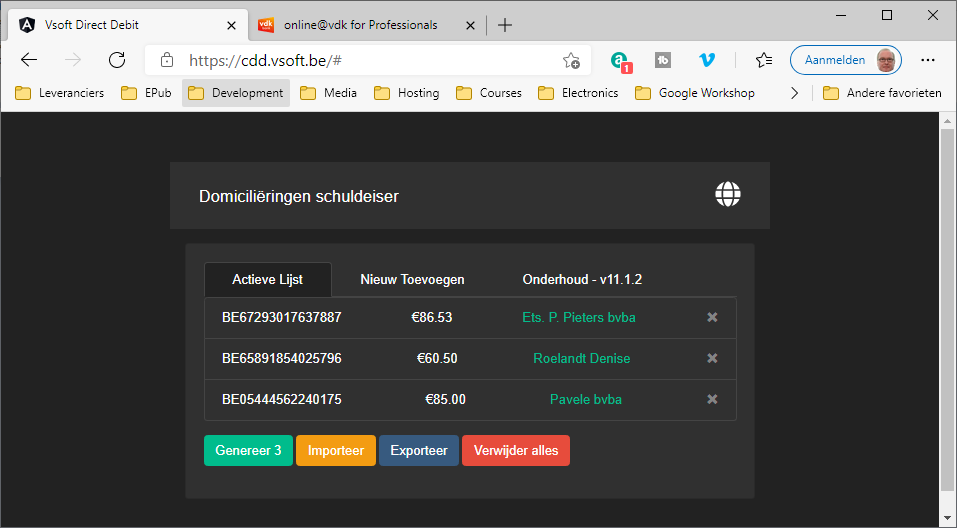
\includegraphics[scale=0.4]{cddscreen}
    \end{center}
    \vspace{0.5em}
  \end{block}
\end{frame}

% [t] for TOP
% \vspace{10pt} for a bit lower vertical
\begin{frame}[t]{Functions}\vspace{10pt}
  \begin{block}{Definition of a block}\vspace{0.5em}
    A function
  \end{block}
\end{frame}

\begin{frame}[t]{Another Title name of my slide}\vspace{10pt}
  \begin{enumerate}
    \item This is item number one
    \item This is item number two
  \end{enumerate}
\end{frame}

\begin{frame}
  hello
\end{frame}

\end{document}

%\usetheme[progressbar = frametitle]{metropolis}
% \setbeamertemplate[frame numbering]{fraction}
%\useoutertheme[]{metropolis}
%\useinnertheme[]{metropolis}
%\usefonttheme[]{metropolis}
%\usecolortheme[]{spruce}
